\subsection{Dark matter subhalos model}
\label{sec:DM_model_chapter}

\subsection{Subhalo J-factors from N-body simulations}
\label{sec:sim-jfactor}
A key component of our pipeline is the so-called ‘J-factor distribution’ of the Galactic subhalo population. This J-factor, also known simply as ‘astrophysical factor’, acts as a normalization factor for the expected annihilation signal and can be computed as the volume integral of the subhalo DM density squared. In this work, we follow ref.~\cite{2024MNRAS.530.2496A} and adopt the J-factor values provided for two different prescriptions of the subhalo internal structure%
\footnote{All data are available at \url{https://projects.ift.uam-csic.es/damasco/?page_id=831}.}: one derived from the mass enclosed within the subhalo tidal radius, $J_\textrm{tidal}^{\Msub}$, and another based on the maximum circular velocity of each subhalo, $J_\textrm{tidal}^{\Vmax}$. 
These two prescriptions are advisable here to estimate current J-factor uncertainties. 
Indeed, measuring subhalo masses is not a trivial task, especially at scales close to the numerical resolution limit of the simulation, where only a few simulation particles are available. Because of this, the computation of masses relies on adopting a specific form of the subhalo DM density profile, which is then fitted to the available simulation data and integrated up to the assumed tidal radius. Unfortunately, even the precise value of the latter can vary significantly among different definitions and is very sensitive to changes in the tidal forces acting on the subhalo as it orbits around the host halo center. In contrast to these mass-related issues, the peak of the circular velocity profile within each subhalo, i.e. $V_{max}$, has been shown to be less affected by numerical resolution and tidal forces (see, e.g., refs.~\cite{2024MNRAS.530.2496A,2025arXiv250601152A}). Its determination also does not depend on adopting a specific functional form of the DM density profile to model the subhalo structural properties. As a result, J-factor calculations based on the latter approach are considered more reliable. Nevertheless, we use both J-factor sets in this study mainly to enable direct comparison with previous results, where J-factor based on subhalo masses are more common. Also, as said, the exercise will  be useful to understand the current level of uncertainties on subhalo modeling.

The calculation of astrophysical J-factors in ref.~\cite{2024MNRAS.530.2496A} is based on the Via Lactea II (VL-II) N-body cosmological simulation \cite{2007ApJ...667..859D}, a DM-only simulation of a Milky-Way-sized halo resolving subhalos down to approximately $10^4$ $\textrm{M}_{\odot}$. 
To explore subhalos below the VL-II resolution limit, 
the simulation was repopulated with millions of smaller subhalos, extending the analysis down by nearly five orders of magnitude 
to about $10^{-1}$ $\textrm{M}_{\odot}$~\cite{2022PhRvD.105h3006C}.
Additionally, by placing the Earth at random positions consistent with its Galactocentric distance, 
thousands of realizations of a Milky Way-like galaxy were created to obtain statistically robust results. 
This led to accurate J-factor distributions (based on both mass and circular velocity) for the entire subhalo population of a galaxy like our own in a $\Lambda$CDM universe. A limitation of ref.~\cite{2024MNRAS.530.2496A} is the absence of baryonic effects in the parent simulation. Baryons are expected to significantly influence the DM subhalo population, particularly in the Galaxy's innermost regions (e.g.,~\cite{2019MNRAS.487.4409K,2017MNRAS.471.1709G,2021MNRAS.501.3558G}), however none of these hydrodynamical simulations resolve subhalos lighter than $\sim 10^6$ $\textrm{M}_{\odot}$. Thus, the survival of such low-mass subhalos to tidal stripping, especially with baryonic influences, remains uncertain~\cite{2018MNRAS.474.3043V,2020MNRAS.491.4591E,2023MNRAS.518...93A}.

In addition to $J_\textrm{tidal}^{\Msub}$ and $J_\textrm{tidal}^{\Vmax}$ from ref.~\cite{2024MNRAS.530.2496A}, we also utilize $J_{0.1}^{\Msub}$ and $J_{0.1}^{\Vmax}$, derived from the same simulation work. These values correspond to J-factors integrated not up to the tidal radius of each subhalo but rather to the corresponding radius subtending 0.1$^\circ$ in the sky. 
This choice aligns with the typical angular resolution of the {\Fermi}-LAT in the GeV range. By using $J_{0.1}^{\Msub}$ and $J_{0.1}^{\Vmax}$, we focus on point-like subhalo emissions, as would appear in \Fermi-LAT point-source catalogs. 
Notably, ref.~\cite{2022PhRvD.105h3006C} concludes that the brightest Galactic subhalos in the \Fermi-LAT gamma-ray sky, if detected, would be extended, with angular sizes around $0.2^\circ$ – $0.3^\circ$. 
Consequently, for such subhalos, our $J_{0.1}^{\Msub}$ and $J_{0.1}^{\Vmax}$ values are expected to be significantly lower than their corresponding $J_\textrm{tidal}^{\Msub}$ and $J_\textrm{tidal}^{\Vmax}$ values. 
We adopt $J_{0.1}^{\Vmax}$ as our nominal case in this paper, while we use the other J-factor values to compare with previous literature, e.g., in Calore et al. (2019)~\cite{2019Galax...7...90C} a $J_{0.1}^{M_\textrm{sub}}$ model was used.

Figure~\ref{fig:Jfactors} illustrates the four sets of J-factor distributions discussed in this section, along with their corresponding number density, which will be the relevant quantity for our pipeline.


\begin{figure}
    \centering
    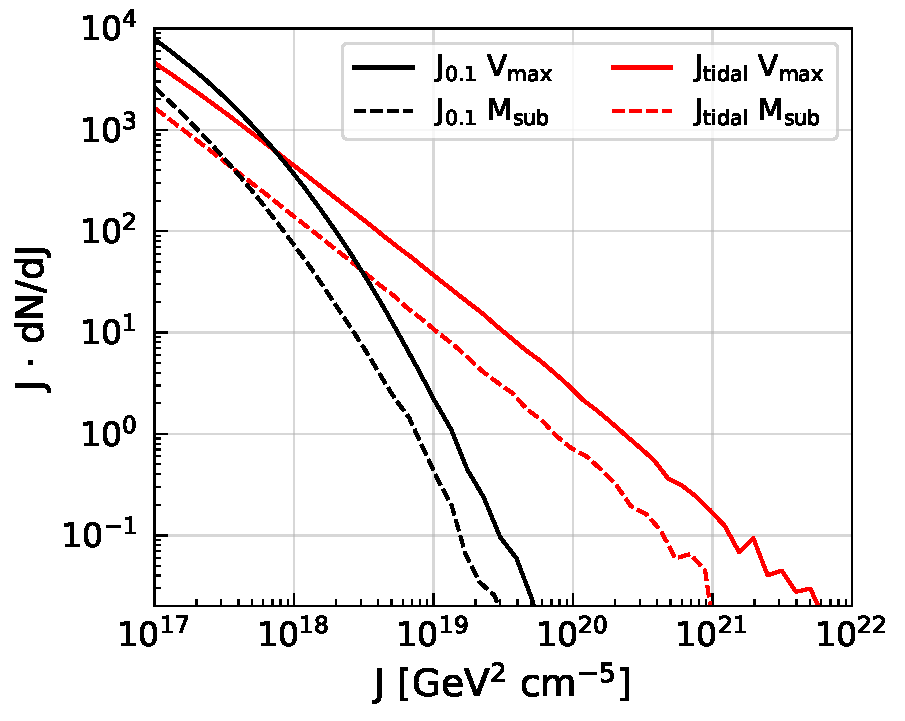
\includegraphics[width=0.5\linewidth]{sections/paper_dm_halos/img/jfactor/Jfactor_number_density_J.pdf}
    \caption{J-factor number density times J for the different J-factor cases considered in this work. See section~\ref{sec:sim-jfactor} for further details.}
    \label{fig:Jfactors}
\end{figure}


\subsection{Gamma-ray emission from dark matter subhalos}
\label{sec:DM_model}





Given a DM setup $\btheta_\textrm{DM}$ (i.e., a DM mass ${\mdm}$, annihilation channel,
and annihilation cross section $\langle\sigma v\rangle$), and an expected distribution of J-factors  determined from DM N-body simulations (described in section \ref{sec:sim-jfactor}), 
we estimate the expected distribution of DM annihilating subhalos that can be detected by {\Fermi} LAT for a certain observation time and instrument response functions (IRFs). 
The procedure is as follows:
\ben
\item
We start with a distribution $p(J) = dN / dJ$ of J-factors expected from N-body DM simulations (cf. figure~\ref{fig:Jfactors} in section~\ref{sec:sim-jfactor}). We sample the values of $J$ from $p(J)$. 
\item
Given a J-factor and DM parameters
$\btheta_\textrm{DM} = \{\langle\sigma v\rangle, {\mdm}, \textrm{ch.}\}$, 
we determine the expected gamma-ray spectrum as
\begin{equation}
\label{eq:DM_spec}
\phi_\textrm{DM}(E;\btheta_\textrm{DM}, J) = \frac{J}{4\pi} \frac{\langle \sigma v \rangle}{2\mdm^2} \left.\frac{dN_\gamma}{dE}\right|_\textrm{ch.},
\end{equation}
where $dN_\gamma/dE$ is the theoretical spectrum of gamma rays produced in an annihilation of a pair of DM particles from ref.~\cite{2024JCAP...03..035A}. 
\item
We place DM subhalos at random positions in the sky with J-factors sampled in step 1 and with the spectra defined in eq.~(\ref{eq:DM_spec}).
\item 
For the diffuse gamma-ray background, we use the official \Fermi-LAT diffuse model template employed in the construction of the 4FGL-DR4 source catalog (\verb|gll_iem_v7|) and the corresponding isotropic background.
\item
We fit the gamma-ray data around each of the simulated DM subhalos with $|b| > 10^\circ$,
where we use the log-parabola model in eq.~(\ref{eq:log_par}) with fitting parameters $\{\log_{10}\phi, \alpha,\beta\}$. 
The fit is performed within a circular region centered on the target DM source. The radius of this region is energy-dependent, corresponding to the 95\% containment angle of the PSF, and is constrained to the range $[0.5^\circ, 5^\circ]$. This range is chosen to ensure sufficient statistics in the highest energy bins while simultaneously avoiding excessive background contamination in the lowest energy bins.
We use the same Gaussian priors for the $\beta$ parameter as in the 4FGL-DR4 catalog with mean 0.1 and sigma 0.3~\cite{2023arXiv230712546B}.
For details see appendix~\ref{app:sim-ps}.
\item
We keep DM subhalos detected with significance TS~$>25$, where $\textrm{TS}=-2\ln \mathcal{L}/\mathcal{L}_*$ is the likelihood-ratio test statistic between the models with and without the subhalo. Such a threshold corresponds to the significance for PS detection in the {\Fermi}-LAT catalogs.
The fraction of subhalos passing the significance cut defines the detection efficiency $\varepsilon_\textrm{eff}(\phi_\textrm{DM})$, which is a function of the DM flux. 
\item
In order to get a good estimate of the DM distribution, $p_\textrm{DM}(\log_{10} \phi_\textrm{DM}, \alpha,\beta|\btheta_\textrm{DM})$, we simulate realizations of the gamma-ray sky until we detect at least 20,000 DM subhalos across all simulations or the number of simulations reaches 1,000. The latter can happen for parameters, where DM subhalos have very small detection probability.%
\footnote{The limit of a thousand simulations is needed to avoid infinite iterations for low-efficiency parameter combinations.
For details on simulation and detection of DM subhalos, see appendix~\ref{app:sim-ps}.
}
\een
In order to reduce the computation time, we perform simulations in flux bins.
At first, we determine the distribution of $\alpha$ and $\beta$ parameters, given the flux $\phi_\textrm{DM}$ and DM parameters $\btheta_\textrm{DM}$, $p_\textrm{DM}(\alpha,\beta|\phi_\textrm{DM};\btheta_\textrm{DM})$, by modeling the distribution of recovered $\alpha$ and $\beta$ parameters in this flux bin (see appendix~\ref{app:sim-ps} for details).
Then we multiply this distribution by the distribution of fluxes, which depends on the distribution of J-factors
$n(\phi_\textrm{DM}) = \frac{dN}{d\phi_\textrm{DM}} (\phi_\textrm{DM};\btheta_\textrm{DM}) = \frac{dN}{dJ} \frac{dJ}{d\phi_\textrm{DM}}$
and by detection efficiency as a function of flux $\varepsilon_\textrm{eff}(\phi_\textrm{DM})$ to determine the probability density times the DM subhalo weight in eq.~(\ref{eq:mixture}):
\begin{equation}
\pi_\textrm{DM}(\btheta_\textrm{DM}) p_\textrm{DM}(\bx;\btheta_\textrm{DM}) = 
\frac{1}{N^\textrm{ROI}_\textrm{unas}}
p_\textrm{DM}(\alpha,\beta|\phi_\textrm{DM};\btheta_\textrm{DM}) 
n(\phi_\textrm{DM})
\varepsilon_\textrm{eff}(\phi_\textrm{DM}),
\label{eq:pDM}
\end{equation}
where $N^\textrm{ROI}_\textrm{unas}$ is the number of unassociated sources in the ROI.

We note that given the DM parameters, the contribution of DM subhalos to unassociated sources is fixed.
In particular, the number of subhalos in our ROI is
\be 
\label{eq:N_ROI}
N^\textrm{ROI}_\textrm{sub}(\btheta_\textrm{DM}) =
\int_\textrm{ROI} d\alpha ~ d\beta ~ d\phi_\textrm{DM}~p_\textrm{DM}(\alpha,\beta|\phi_\textrm{DM};\btheta_\textrm{DM}) ~n(\phi_\textrm{DM}) \varepsilon_\textrm{eff}(\phi_\textrm{DM}),
\ee
while the DM weight $\pi_\textrm{DM}$ in eq.~(\ref{eq:mixture}) is 
\be
\pi_\textrm{DM}(\btheta_\textrm{DM}) = \frac{N^\textrm{ROI}_\textrm{sub}(\btheta_\textrm{DM})}{N^\textrm{ROI}_\textrm{unas}}.
\ee

In figure~\ref{fig:dmdist-all} we show the distributions of DM subhalos in $\alpha$ and $\beta$ parameters (we integrate the distributions in the flux dimension for presentation purposes) for different DM masses at some characteristic $\langle\sigma v\rangle$ values. 
We note that the DM distributions are not fully contained inside the  ROI that we selected in this analysis, which is indicated as a green box in the plots. 

In particular, a significant fraction of the DM subhalo distribution is truncated for DM masses of 10 GeV, 30 GeV, and 1 TeV.
\old{For these masses our analysis can be further improved by adopting a covariate shift model suitable for a larger region in feature space.}
\new{Although choosing a larger ROI that covers a larger fraction of the DM subhalo distribution could increase statistics, our assumption that the covariate shift can be modeled by a monotonous function would not be valid anymore. Introducing a more flexible covariate shift model to account for this would require additional parameters, potentially leading to larger uncertainty in $\pi_\textrm{DM}$ due to correlations with these new parameters (i.e., a larger parameter covariance matrix) and, consequently, weaker limits. Moreover, the gain from larger statistics would be limited by the significant background of astrophysical sources outside of our current ROI, particularly unassociated millisecond pulsars with $\alpha > 0.7$ and $\beta \sim 0.4$ (upper right panel of figure~\ref{fig:dmdist-all}). Conversely, regions with small $\alpha$ values (bottom panel) contain very few astrophysical sources, necessitating extrapolation that carries large systematic uncertainties (see the wide uncertainty band for small alpha values in the upper left panel in figure~\ref{fig:dist_ratio}). Finally, our limits on DM annihilation are conservative: positive residuals after fitting the data with astrophysical components can be absorbed by the DM component, resulting in a positive best-fit $\pi_\textrm{DM}$ and weaker upper limits than in the $\pi_\textrm{DM} = 0$ case.}

\begin{figure}
    \centering
    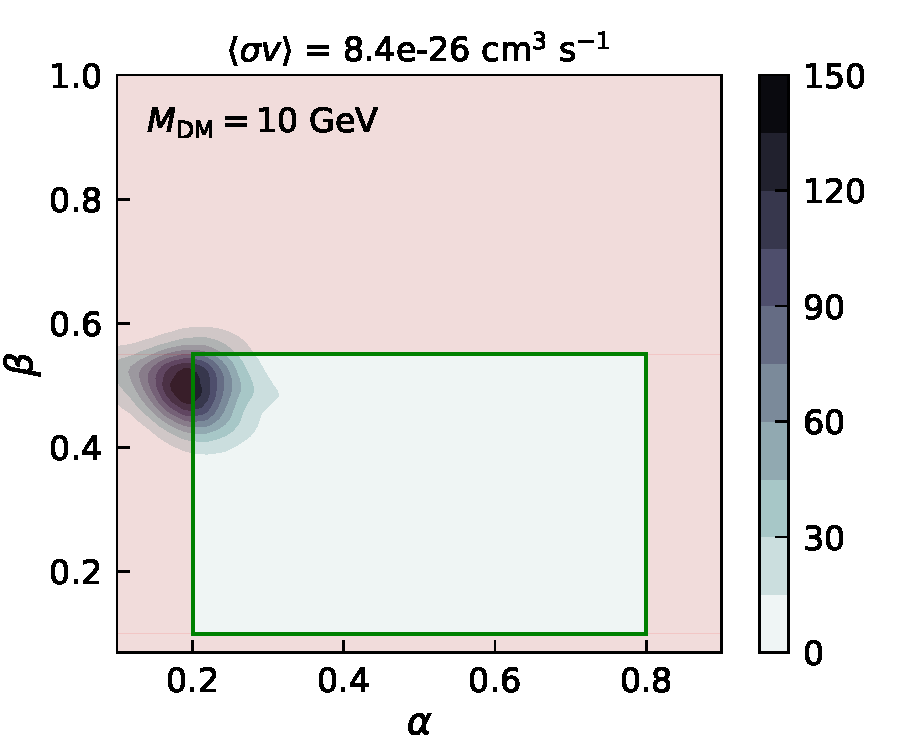
\includegraphics[width=0.45\linewidth]{sections/paper_dm_halos/img/dm_dist/pDM_integrated_mDM_10_GeV.pdf}
    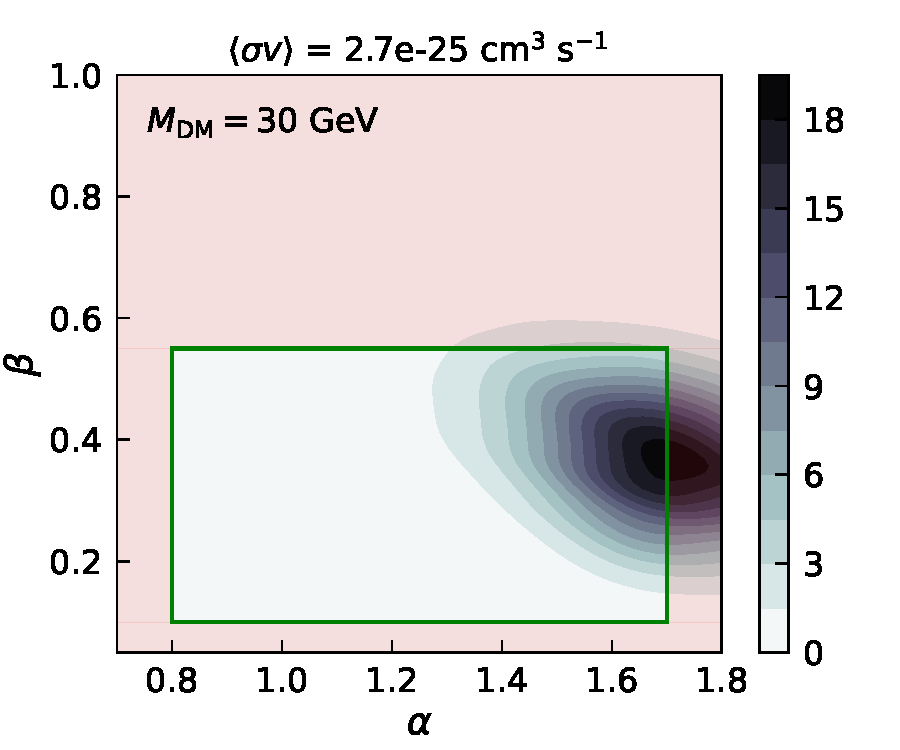
\includegraphics[width=0.45\linewidth]{sections/paper_dm_halos/img/dm_dist/pDM_integrated_mDM_30_GeV.pdf}
    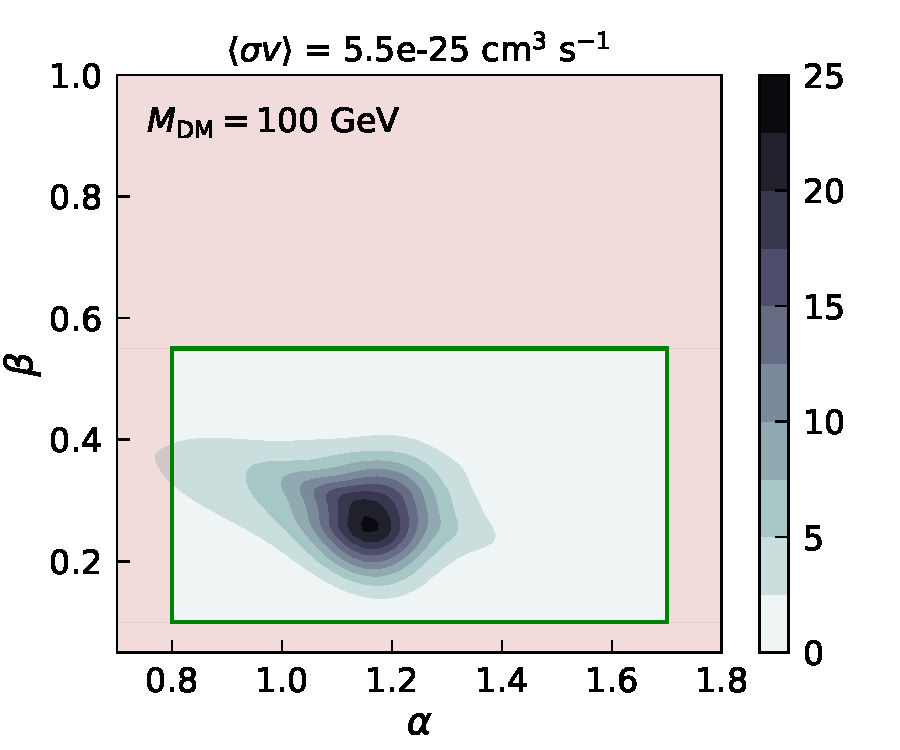
\includegraphics[width=0.45\linewidth]{sections/paper_dm_halos/img/dm_dist/pDM_integrated_mDM_100_GeV.pdf}
    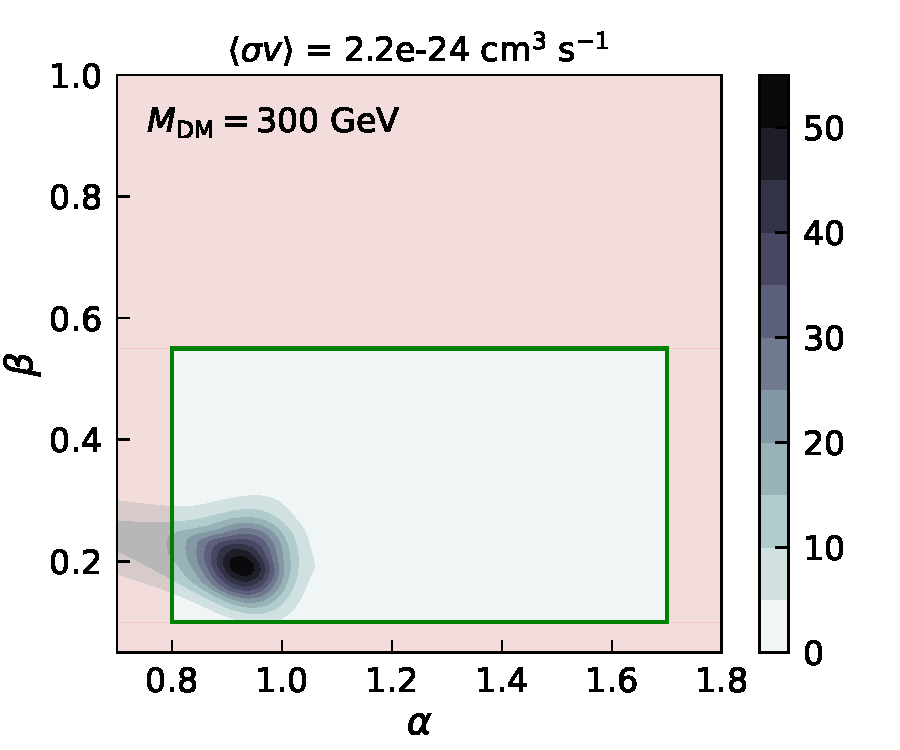
\includegraphics[width=0.45\linewidth]{sections/paper_dm_halos/img/dm_dist/pDM_integrated_mDM_300_GeV.pdf}
    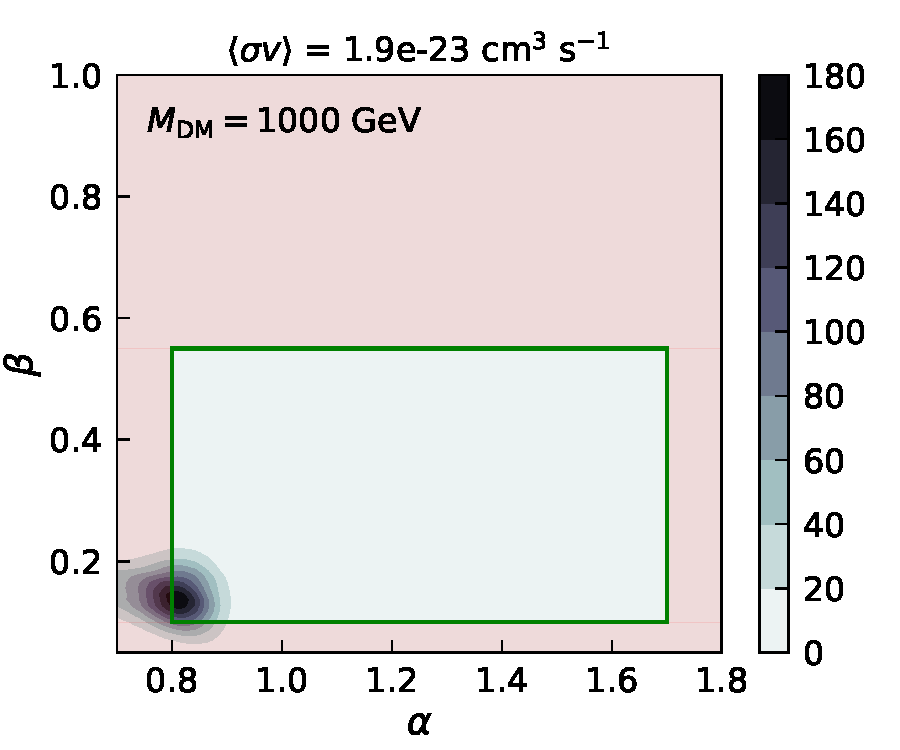
\includegraphics[width=0.45\linewidth]{sections/paper_dm_halos/img/dm_dist/pDM_integrated_mDM_1000_GeV.pdf}
    \caption{DM distribution at different DM masses, $b\overline{b}$ annihilation channel, integrated in flux for visualization purposes. The $\langle\sigma v\rangle$ values are chosen close to our bound values. 
    The green boxes indicate the parameter ranges (ROI) used for this analysis and define the truncation region for the distribution. The color bars show the value of the DM subhalo PDF (eq. \ref{eq:pDM}), normalized to unit integral within the ROI.
    }
    \label{fig:dmdist-all}
\end{figure}

\begin{figure}
    \centering
    \resizebox{0.95\textwidth}{!}{
    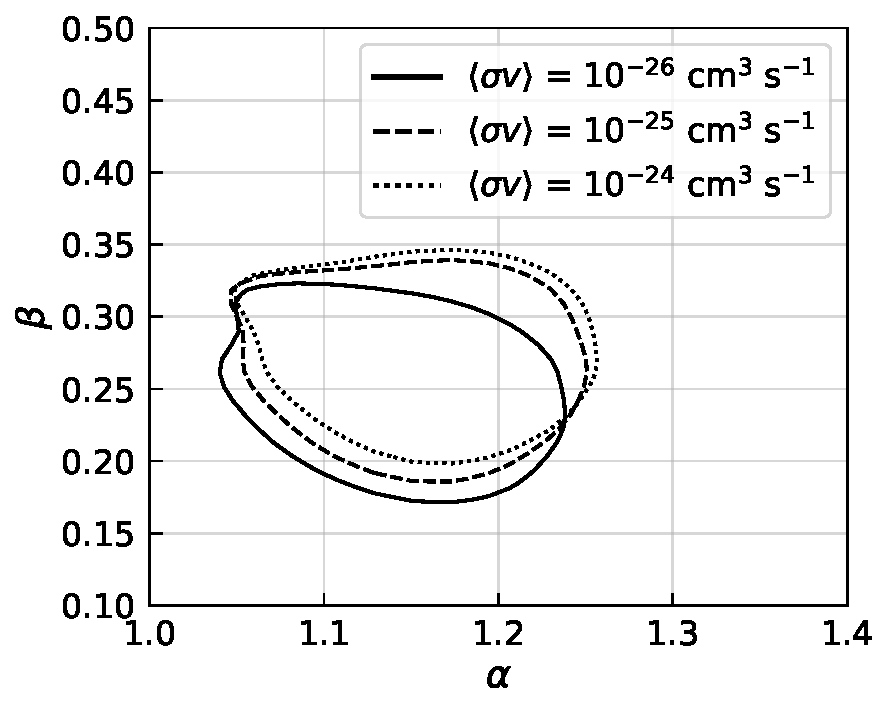
\includegraphics[width=0.49\linewidth]{sections/paper_dm_halos/img/dm_dist_countour/pDM_integrated_mDM_100_GeV_sigmav.pdf}
    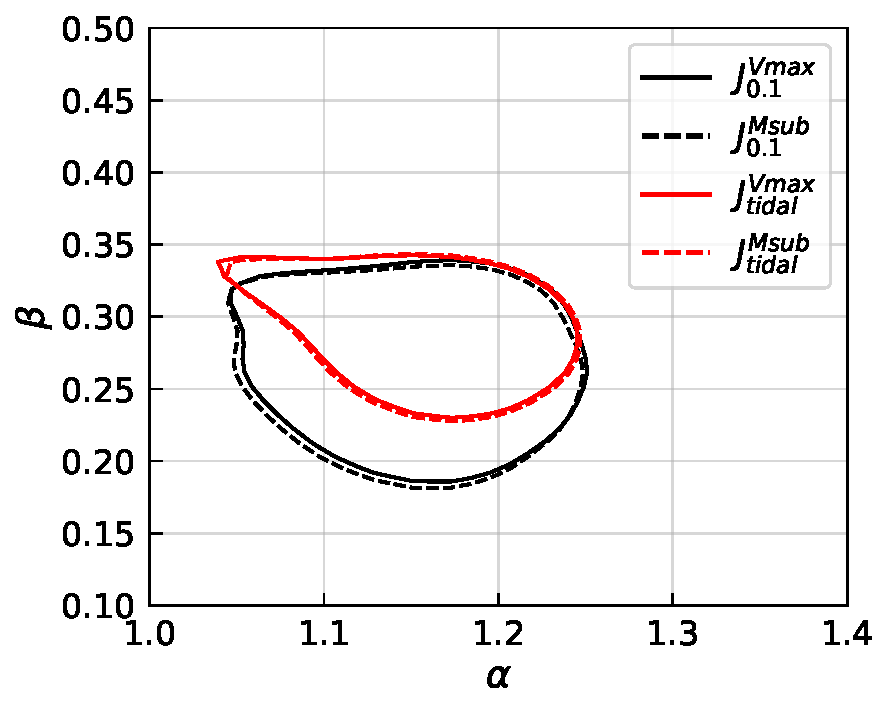
\includegraphics[width=0.49\linewidth]{sections/paper_dm_halos/img/dm_dist_countour/pDM_integrated_mDM_100_GeV_J_factor.pdf}
    }
    \caption{Contour plots at half maximum of the DM subhalo distribution for different values of $\sigmav$ and J-factor models at $\mdm$ = 100 GeV. \panel{Left panel}: contour lines for different choices of $\sigmav$ for $J_{0.1}^{Vmax}$. 
    \panel{Right panel}: contour lines for different J-factor models for $\sigmav = 10^{-25}$ $\textrm{cm}^{3} \, \textrm{s}^{-1}$.}
    \label{fig:DM_dist_countour}
\end{figure}


In figure~\ref{fig:DM_dist_countour} we show the contour levels for the half maximum of the DM subhalo distribution for different choices of $\sigmav$ and J-factor models for $\mdm$ = 100 GeV. 
The distribution shifts to higher values of $\beta$ for larger $\sigmav$ values. Analogously, choosing $J_{tidal}$ shifts the distribution to higher $\beta$ values compared to $J_{0.1}$.
This is to be expected, since for faint sources (small $\sigmav$ or small J-factors) the fit has large statistical uncertainties and the best-fit value of the $\beta$ parameter is more affected by the priors on $\beta$ than in case of bright sources.

